\documentclass[1p]{elsarticle_modified}
%\bibliographystyle{elsarticle-num}

%\usepackage[colorlinks]{hyperref}
%\usepackage{abbrmath_seonhwa} %\Abb, \Ascr, \Acal ,\Abf, \Afrak
\usepackage{amsfonts}
\usepackage{amssymb}
\usepackage{amsmath}
\usepackage{amsthm}
\usepackage{scalefnt}
\usepackage{amsbsy}
\usepackage{kotex}
\usepackage{caption}
\usepackage{subfig}
\usepackage{color}
\usepackage{graphicx}
\usepackage{xcolor} %% white, black, red, green, blue, cyan, magenta, yellow
\usepackage{float}
\usepackage{setspace}
\usepackage{hyperref}

\usepackage{tikz}
\usetikzlibrary{arrows}

\usepackage{multirow}
\usepackage{array} % fixed length table
\usepackage{hhline}

%%%%%%%%%%%%%%%%%%%%%
\makeatletter
\renewcommand*\env@matrix[1][\arraystretch]{%
	\edef\arraystretch{#1}%
	\hskip -\arraycolsep
	\let\@ifnextchar\new@ifnextchar
	\array{*\c@MaxMatrixCols c}}
\makeatother %https://tex.stackexchange.com/questions/14071/how-can-i-increase-the-line-spacing-in-a-matrix
%%%%%%%%%%%%%%%

\usepackage[normalem]{ulem}

\newcommand{\msout}[1]{\ifmmode\text{\sout{\ensuremath{#1}}}\else\sout{#1}\fi}
%SOURCE: \msout is \stkout macro in https://tex.stackexchange.com/questions/20609/strikeout-in-math-mode

\newcommand{\cancel}[1]{
	\ifmmode
	{\color{red}\msout{#1}}
	\else
	{\color{red}\sout{#1}}
	\fi
}

\newcommand{\add}[1]{
	{\color{blue}\uwave{#1}}
}

\newcommand{\replace}[2]{
	\ifmmode
	{\color{red}\msout{#1}}{\color{blue}\uwave{#2}}
	\else
	{\color{red}\sout{#1}}{\color{blue}\uwave{#2}}
	\fi
}

\newcommand{\Sol}{\mathcal{S}} %segment
\newcommand{\D}{D} %diagram
\newcommand{\A}{\mathcal{A}} %arc


%%%%%%%%%%%%%%%%%%%%%%%%%%%%%5 test

\def\sl{\operatorname{\textup{SL}}(2,\Cbb)}
\def\psl{\operatorname{\textup{PSL}}(2,\Cbb)}
\def\quan{\mkern 1mu \triangleright \mkern 1mu}

\theoremstyle{definition}
\newtheorem{thm}{Theorem}[section]
\newtheorem{prop}[thm]{Proposition}
\newtheorem{lem}[thm]{Lemma}
\newtheorem{ques}[thm]{Question}
\newtheorem{cor}[thm]{Corollary}
\newtheorem{defn}[thm]{Definition}
\newtheorem{exam}[thm]{Example}
\newtheorem{rmk}[thm]{Remark}
\newtheorem{alg}[thm]{Algorithm}

\newcommand{\I}{\sqrt{-1}}
\begin{document}

%\begin{frontmatter}
%
%\title{Boundary parabolic representations of knots up to 8 crossings}
%
%%% Group authors per affiliation:
%\author{Yunhi Cho} 
%\address{Department of Mathematics, University of Seoul, Seoul, Korea}
%\ead{yhcho@uos.ac.kr}
%
%
%\author{Seonhwa Kim} %\fnref{s_kim}}
%\address{Center for Geometry and Physics, Institute for Basic Science, Pohang, 37673, Korea}
%\ead{ryeona17@ibs.re.kr}
%
%\author{Hyuk Kim}
%\address{Department of Mathematical Sciences, Seoul National University, Seoul 08826, Korea}
%\ead{hyukkim@snu.ac.kr}
%
%\author{Seokbeom Yoon}
%\address{Department of Mathematical Sciences, Seoul National University, Seoul, 08826,  Korea}
%\ead{sbyoon15@snu.ac.kr}
%
%\begin{abstract}
%We find all boundary parabolic representation of knots up to 8 crossings.
%
%\end{abstract}
%\begin{keyword}
%    \MSC[2010] 57M25 
%\end{keyword}
%
%\end{frontmatter}

%\linenumbers
%\tableofcontents
%
\newcommand\colored[1]{\textcolor{white}{\rule[-0.35ex]{0.8em}{1.4ex}}\kern-0.8em\color{red} #1}%
%\newcommand\colored[1]{\textcolor{white}{ #1}\kern-2.17ex	\textcolor{white}{ #1}\kern-1.81ex	\textcolor{white}{ #1}\kern-2.15ex\color{red}#1	}

{\Large $\underline{12a_{1173}~(K12a_{1173})}$}

\setlength{\tabcolsep}{10pt}
\renewcommand{\arraystretch}{1.6}
\vspace{1cm}\begin{tabular}{m{100pt}>{\centering\arraybackslash}m{274pt}}
\multirow{5}{120pt}{
	\centering
	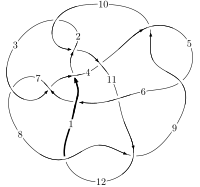
\includegraphics[width=112pt]{../../../GIT/diagram.site/Diagrams/png/1974_12a_1173.png}\\
\ \ \ A knot diagram\footnotemark}&
\allowdisplaybreaks
\textbf{Linearized knot diagam} \\
\cline{2-2}
 &
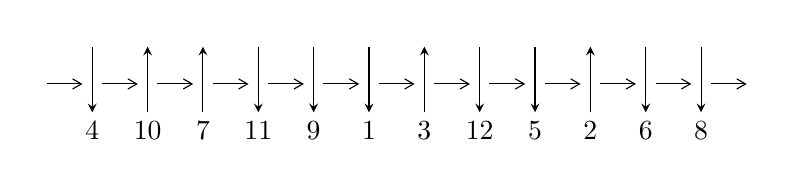
\begin{tikzpicture}[x=20pt, y=17pt]
	% nodes
	\node (C0) at (0, 0) {};
	\node (C1) at (1, 0) {};
	\node (C1U) at (1, +1) {};
	\node (C1D) at (1, -1) {4};

	\node (C2) at (2, 0) {};
	\node (C2U) at (2, +1) {};
	\node (C2D) at (2, -1) {10};

	\node (C3) at (3, 0) {};
	\node (C3U) at (3, +1) {};
	\node (C3D) at (3, -1) {7};

	\node (C4) at (4, 0) {};
	\node (C4U) at (4, +1) {};
	\node (C4D) at (4, -1) {11};

	\node (C5) at (5, 0) {};
	\node (C5U) at (5, +1) {};
	\node (C5D) at (5, -1) {9};

	\node (C6) at (6, 0) {};
	\node (C6U) at (6, +1) {};
	\node (C6D) at (6, -1) {1};

	\node (C7) at (7, 0) {};
	\node (C7U) at (7, +1) {};
	\node (C7D) at (7, -1) {3};

	\node (C8) at (8, 0) {};
	\node (C8U) at (8, +1) {};
	\node (C8D) at (8, -1) {12};

	\node (C9) at (9, 0) {};
	\node (C9U) at (9, +1) {};
	\node (C9D) at (9, -1) {5};

	\node (C10) at (10, 0) {};
	\node (C10U) at (10, +1) {};
	\node (C10D) at (10, -1) {2};

	\node (C11) at (11, 0) {};
	\node (C11U) at (11, +1) {};
	\node (C11D) at (11, -1) {6};

	\node (C12) at (12, 0) {};
	\node (C12U) at (12, +1) {};
	\node (C12D) at (12, -1) {8};
	\node (C13) at (13, 0) {};

	% arrows
	\draw[->,>={angle 60}]
	(C0) edge (C1) (C1) edge (C2) (C2) edge (C3) (C3) edge (C4) (C4) edge (C5) (C5) edge (C6) (C6) edge (C7) (C7) edge (C8) (C8) edge (C9) (C9) edge (C10) (C10) edge (C11) (C11) edge (C12) (C12) edge (C13) ;	\draw[->,>=stealth]
	(C1U) edge (C1D) (C2D) edge (C2U) (C3D) edge (C3U) (C4U) edge (C4D) (C5U) edge (C5D) (C6U) edge (C6D) (C7D) edge (C7U) (C8U) edge (C8D) (C9U) edge (C9D) (C10D) edge (C10U) (C11U) edge (C11D) (C12U) edge (C12D) ;
	\end{tikzpicture} \\
\hhline{~~} \\& 
\textbf{Solving Sequence} \\ \cline{2-2} 
 &
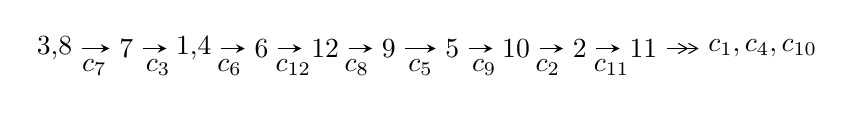
\begin{tikzpicture}[x=23pt, y=7pt]
	% node
	\node (A0) at (-1/8, 0) {3,8};
	\node (A1) at (1, 0) {7};
	\node (A2) at (33/16, 0) {1,4};
	\node (A3) at (25/8, 0) {6};
	\node (A4) at (33/8, 0) {12};
	\node (A5) at (41/8, 0) {9};
	\node (A6) at (49/8, 0) {5};
	\node (A7) at (57/8, 0) {10};
	\node (A8) at (65/8, 0) {2};
	\node (A9) at (73/8, 0) {11};
	\node (C1) at (1/2, -1) {$c_{7}$};
	\node (C2) at (3/2, -1) {$c_{3}$};
	\node (C3) at (21/8, -1) {$c_{6}$};
	\node (C4) at (29/8, -1) {$c_{12}$};
	\node (C5) at (37/8, -1) {$c_{8}$};
	\node (C6) at (45/8, -1) {$c_{5}$};
	\node (C7) at (53/8, -1) {$c_{9}$};
	\node (C8) at (61/8, -1) {$c_{2}$};
	\node (C9) at (69/8, -1) {$c_{11}$};
	\node (A10) at (11, 0) {$c_{1},c_{4},c_{10}$};

	% edge
	\draw[->,>=stealth]	
	(A0) edge (A1) (A1) edge (A2) (A2) edge (A3) (A3) edge (A4) (A4) edge (A5) (A5) edge (A6) (A6) edge (A7) (A7) edge (A8) (A8) edge (A9) ;
	\draw[->>,>={angle 60}]	
	(A9) edge (A10);
\end{tikzpicture} \\ 

\end{tabular} \\

\footnotetext{
The image of knot diagram is generated by the software ``\textbf{Draw programme}" developed by Andrew Bartholomew(\url{http://www.layer8.co.uk/maths/draw/index.htm\#Running-draw}), where we modified some parts for our purpose(\url{https://github.com/CATsTAILs/LinksPainter}).
}\phantom \\ \newline 
\centering \textbf{Ideals for irreducible components\footnotemark of $X_{\text{par}}$} 
 
\begin{align*}
I^u_{1}&=\langle 
-115544486760242 u^{28}+112064365539712 u^{27}+\cdots+3495407185462 b-11587431516889,\\
\phantom{I^u_{1}}&\phantom{= \langle  }244809699887266 u^{28}-271674151669112 u^{27}+\cdots+10486221556386 a+8547110162663,\\
\phantom{I^u_{1}}&\phantom{= \langle  }2 u^{29}-2 u^{28}+\cdots+u+1\rangle \\
I^u_{2}&=\langle 
-1.17039\times10^{521} u^{113}-2.71734\times10^{521} u^{112}+\cdots+6.71963\times10^{521} b+1.06384\times10^{525},\\
\phantom{I^u_{2}}&\phantom{= \langle  }1.20930\times10^{526} u^{113}+4.51340\times10^{526} u^{112}+\cdots+7.27729\times10^{526} a+9.87445\times10^{530},\\
\phantom{I^u_{2}}&\phantom{= \langle  }2 u^{114}+6 u^{113}+\cdots+736731 u+108299\rangle \\
I^u_{3}&=\langle 
-78 u^9-66 u^8-309 u^7-66 u^6-467 u^5-40 u^4-324 u^3+16 u^2+23 b-118 u+11,\\
\phantom{I^u_{3}}&\phantom{= \langle  }50 u^9+60 u^8+191 u^7+83 u^6+228 u^5+74 u^4+121 u^3-2 u^2+23 a+55 u-10,\\
\phantom{I^u_{3}}&\phantom{= \langle  }2 u^{10}+2 u^9+9 u^8+4 u^7+16 u^6+5 u^5+14 u^4+3 u^3+7 u^2+u+1\rangle \\
I^u_{4}&=\langle 
3331518 u^{17}+402774 u^{16}+\cdots+504688 b-1213603,\\
\phantom{I^u_{4}}&\phantom{= \langle  }10659510 u^{17}+6709470 u^{16}+\cdots+504688 a+4961241,\;2 u^{18}+6 u^{16}+\cdots-3 u+1\rangle \\
\\
\end{align*}
\raggedright * 4 irreducible components of $\dim_{\mathbb{C}}=0$, with total 171 representations.\\
\footnotetext{All coefficients of polynomials are rational numbers. But the coefficients are sometimes approximated in decimal forms when there is not enough margin.}
\newpage
\renewcommand{\arraystretch}{1}
\centering \section*{I. $I^u_{1}= \langle -1.16\times10^{14} u^{28}+1.12\times10^{14} u^{27}+\cdots+3.50\times10^{12} b-1.16\times10^{13},\;2.45\times10^{14} u^{28}-2.72\times10^{14} u^{27}+\cdots+1.05\times10^{13} a+8.55\times10^{12},\;2 u^{29}-2 u^{28}+\cdots+u+1 \rangle$}
\flushleft \textbf{(i) Arc colorings}\\
\begin{tabular}{m{7pt} m{180pt} m{7pt} m{180pt} }
\flushright $a_{3}=$&$\begin{pmatrix}0\\u\end{pmatrix}$ \\
\flushright $a_{8}=$&$\begin{pmatrix}1\\0\end{pmatrix}$ \\
\flushright $a_{7}=$&$\begin{pmatrix}1\\u^2\end{pmatrix}$ \\
\flushright $a_{1}=$&$\begin{pmatrix}-23.3458 u^{28}+25.9077 u^{27}+\cdots-24.2799 u-0.815080\\33.0561 u^{28}-32.0605 u^{27}+\cdots+36.7864 u+3.31504\end{pmatrix}$ \\
\flushright $a_{4}=$&$\begin{pmatrix}u\\u^3+u\end{pmatrix}$ \\
\flushright $a_{6}=$&$\begin{pmatrix}6.98329 u^{28}-3.30384 u^{27}+\cdots+5.42111 u+3.00882\\5.19262 u^{28}-30.1366 u^{27}+\cdots-9.99582 u-22.2338\end{pmatrix}$ \\
\flushright $a_{12}=$&$\begin{pmatrix}9.71024 u^{28}-6.15274 u^{27}+\cdots+12.5066 u+2.49996\\33.0561 u^{28}-32.0605 u^{27}+\cdots+36.7864 u+3.31504\end{pmatrix}$ \\
\flushright $a_{9}=$&$\begin{pmatrix}-6.54769 u^{28}+34.9638 u^{27}+\cdots+13.3331 u+27.2899\\-9.17085 u^{28}+32.9069 u^{27}+\cdots+6.34418 u+19.8937\end{pmatrix}$ \\
\flushright $a_{5}=$&$\begin{pmatrix}-9.71024 u^{28}+6.15274 u^{27}+\cdots-12.5066 u-2.49996\\-44.2855 u^{28}+32.3420 u^{27}+\cdots-56.2713 u-16.4508\end{pmatrix}$ \\
\flushright $a_{10}=$&$\begin{pmatrix}1\\10.8221 u^{28}-55.7517 u^{27}+\cdots-25.3655 u-43.2633\end{pmatrix}$ \\
\flushright $a_{2}=$&$\begin{pmatrix}- u\\44.9296 u^{28}-43.2994 u^{27}+\cdots+49.6743 u+5.41107\end{pmatrix}$ \\
\flushright $a_{11}=$&$\begin{pmatrix}- u^2-1\\-9.19197 u^{28}+30.7757 u^{27}+\cdots+8.31175 u+20.7985\end{pmatrix}$\\&\end{tabular}
\flushleft \textbf{(ii) Obstruction class $= -1$}\\~\\
\flushleft \textbf{(iii) Cusp Shapes $= -\frac{182509966010848}{1747703592731} u^{28}+\frac{211508404855216}{1747703592731} u^{27}+\cdots-\frac{167107576397767}{1747703592731} u-\frac{1848186597135}{1747703592731}$}\\~\\
\newpage\renewcommand{\arraystretch}{1}
\flushleft \textbf{(iv) u-Polynomials at the component}\newline \\
\begin{tabular}{m{50pt}|m{274pt}}
Crossings & \hspace{64pt}u-Polynomials at each crossing \\
\hline $$\begin{aligned}c_{1}\end{aligned}$$&$\begin{aligned}
&u^{29}-7 u^{28}+\cdots+288 u-88
\end{aligned}$\\
\hline $$\begin{aligned}c_{2},c_{3},c_{7}\\c_{10}\end{aligned}$$&$\begin{aligned}
&2(2 u^{29}-2 u^{28}+\cdots+u+1)
\end{aligned}$\\
\hline $$\begin{aligned}c_{4},c_{6}\end{aligned}$$&$\begin{aligned}
&u^{29}+2 u^{28}+\cdots+28 u+2
\end{aligned}$\\
\hline $$\begin{aligned}c_{5},c_{8},c_{9}\\c_{12}\end{aligned}$$&$\begin{aligned}
&u^{29}+14 u^{27}+\cdots+7 u+1
\end{aligned}$\\
\hline $$\begin{aligned}c_{11}\end{aligned}$$&$\begin{aligned}
&4(4 u^{29}+80 u^{28}+\cdots+1844 u+104)
\end{aligned}$\\
\hline
\end{tabular}\\~\\
\newpage\renewcommand{\arraystretch}{1}
\flushleft \textbf{(v) Riley Polynomials at the component}\newline \\
\begin{tabular}{m{50pt}|m{274pt}}
Crossings & \hspace{64pt}Riley Polynomials at each crossing \\
\hline $$\begin{aligned}c_{1}\end{aligned}$$&$\begin{aligned}
&y^{29}-13 y^{28}+\cdots+2336 y-7744
\end{aligned}$\\
\hline $$\begin{aligned}c_{2},c_{3},c_{7}\\c_{10}\end{aligned}$$&$\begin{aligned}
&4(4 y^{29}+56 y^{28}+\cdots-11 y-1)
\end{aligned}$\\
\hline $$\begin{aligned}c_{4},c_{6}\end{aligned}$$&$\begin{aligned}
&y^{29}-2 y^{28}+\cdots+156 y-4
\end{aligned}$\\
\hline $$\begin{aligned}c_{5},c_{8},c_{9}\\c_{12}\end{aligned}$$&$\begin{aligned}
&y^{29}+28 y^{28}+\cdots-23 y-1
\end{aligned}$\\
\hline $$\begin{aligned}c_{11}\end{aligned}$$&$\begin{aligned}
&16(16 y^{29}-24 y^{28}+\cdots-5040 y-10816)
\end{aligned}$\\
\hline
\end{tabular}\\~\\
\newpage\flushleft \textbf{(vi) Complex Volumes and Cusp Shapes}
$$\begin{array}{c|c|c}  
\text{Solutions to }I^u_{1}& \I (\text{vol} + \sqrt{-1}CS) & \text{Cusp shape}\\
 \hline 
\begin{aligned}
u &= \phantom{-}0.614826 + 0.850857 I \\
a &= -1.81142 - 0.42202 I \\
b &= -0.032852 - 1.262430 I\end{aligned}
 & \phantom{-}4.41811 + 4.54585 I & -0.45562 - 6.52820 I \\ \hline\begin{aligned}
u &= \phantom{-}0.614826 - 0.850857 I \\
a &= -1.81142 + 0.42202 I \\
b &= -0.032852 + 1.262430 I\end{aligned}
 & \phantom{-}4.41811 - 4.54585 I & -0.45562 + 6.52820 I \\ \hline\begin{aligned}
u &= \phantom{-}0.655035 + 0.842071 I \\
a &= -1.107760 - 0.777899 I \\
b &= \phantom{-}0.21309 - 1.41045 I\end{aligned}
 & \phantom{-}4.65613 + 5.31778 I & \phantom{-}0.68850 - 5.52713 I \\ \hline\begin{aligned}
u &= \phantom{-}0.655035 - 0.842071 I \\
a &= -1.107760 + 0.777899 I \\
b &= \phantom{-}0.21309 + 1.41045 I\end{aligned}
 & \phantom{-}4.65613 - 5.31778 I & \phantom{-}0.68850 + 5.52713 I \\ \hline\begin{aligned}
u &= -0.523123 + 0.947153 I \\
a &= \phantom{-}2.24569 + 0.18671 I \\
b &= -0.57260 - 1.42544 I\end{aligned}
 & \phantom{-}4.95066 - 10.99740 I & -2.56166 + 11.07052 I \\ \hline\begin{aligned}
u &= -0.523123 - 0.947153 I \\
a &= \phantom{-}2.24569 - 0.18671 I \\
b &= -0.57260 + 1.42544 I\end{aligned}
 & \phantom{-}4.95066 + 10.99740 I & -2.56166 - 11.07052 I \\ \hline\begin{aligned}
u &= \phantom{-}1.075760 + 0.138675 I \\
a &= -0.175885 + 0.502122 I \\
b &= \phantom{-}0.352141 + 1.353960 I\end{aligned}
 & \phantom{-}7.43832 - 7.27144 I & \phantom{-}1.54133 + 6.09063 I \\ \hline\begin{aligned}
u &= \phantom{-}1.075760 - 0.138675 I \\
a &= -0.175885 - 0.502122 I \\
b &= \phantom{-}0.352141 - 1.353960 I\end{aligned}
 & \phantom{-}7.43832 + 7.27144 I & \phantom{-}1.54133 - 6.09063 I \\ \hline\begin{aligned}
u &= -0.415146 + 0.770962 I \\
a &= \phantom{-}1.45156 - 1.38441 I \\
b &= -0.123319 - 0.160384 I\end{aligned}
 & -5.19900 - 3.27887 I & -11.5569 - 9.3645 I \\ \hline\begin{aligned}
u &= -0.415146 - 0.770962 I \\
a &= \phantom{-}1.45156 + 1.38441 I \\
b &= -0.123319 + 0.160384 I\end{aligned}
 & -5.19900 + 3.27887 I & -11.5569 + 9.3645 I\\
 \hline 
 \end{array}$$\newpage$$\begin{array}{c|c|c}  
\text{Solutions to }I^u_{1}& \I (\text{vol} + \sqrt{-1}CS) & \text{Cusp shape}\\
 \hline 
\begin{aligned}
u &= \phantom{-}0.227409 + 0.725395 I \\
a &= -1.31024 - 1.59568 I \\
b &= \phantom{-}0.516550 + 1.035240 I\end{aligned}
 & \phantom{-}0.017310 + 0.877054 I & -1.61037 - 4.73307 I \\ \hline\begin{aligned}
u &= \phantom{-}0.227409 - 0.725395 I \\
a &= -1.31024 + 1.59568 I \\
b &= \phantom{-}0.516550 - 1.035240 I\end{aligned}
 & \phantom{-}0.017310 - 0.877054 I & -1.61037 + 4.73307 I \\ \hline\begin{aligned}
u &= -0.025164 + 0.735565 I \\
a &= \phantom{-}0.43474 - 1.50702 I \\
b &= -0.513005 + 0.763820 I\end{aligned}
 & -0.77973 + 1.38398 I & -8.48794 - 5.27599 I \\ \hline\begin{aligned}
u &= -0.025164 - 0.735565 I \\
a &= \phantom{-}0.43474 + 1.50702 I \\
b &= -0.513005 - 0.763820 I\end{aligned}
 & -0.77973 - 1.38398 I & -8.48794 + 5.27599 I \\ \hline\begin{aligned}
u &= -0.059260 + 0.726815 I \\
a &= -0.282978 + 0.091872 I \\
b &= \phantom{-}0.25912 - 1.55543 I\end{aligned}
 & \phantom{-}7.47471 + 4.30695 I & -11.81657 - 0.82827 I \\ \hline\begin{aligned}
u &= -0.059260 - 0.726815 I \\
a &= -0.282978 - 0.091872 I \\
b &= \phantom{-}0.25912 + 1.55543 I\end{aligned}
 & \phantom{-}7.47471 - 4.30695 I & -11.81657 + 0.82827 I \\ \hline\begin{aligned}
u &= -0.710709 + 0.024669 I \\
a &= \phantom{-}0.487463 + 0.385541 I \\
b &= \phantom{-}0.250282 + 1.341540 I\end{aligned}
 & \phantom{-}8.75165 - 3.48954 I & \phantom{-}8.31054 + 1.44290 I \\ \hline\begin{aligned}
u &= -0.710709 - 0.024669 I \\
a &= \phantom{-}0.487463 - 0.385541 I \\
b &= \phantom{-}0.250282 - 1.341540 I\end{aligned}
 & \phantom{-}8.75165 + 3.48954 I & \phantom{-}8.31054 - 1.44290 I \\ \hline\begin{aligned}
u &= -0.459295 + 1.237870 I \\
a &= -1.184610 + 0.482592 I \\
b &= \phantom{-}1.000480 - 0.171236 I\end{aligned}
 & -7.99683 - 8.14911 I & -10.73836 + 6.19923 I \\ \hline\begin{aligned}
u &= -0.459295 - 1.237870 I \\
a &= -1.184610 - 0.482592 I \\
b &= \phantom{-}1.000480 + 0.171236 I\end{aligned}
 & -7.99683 + 8.14911 I & -10.73836 - 6.19923 I\\
 \hline 
 \end{array}$$\newpage$$\begin{array}{c|c|c}  
\text{Solutions to }I^u_{1}& \I (\text{vol} + \sqrt{-1}CS) & \text{Cusp shape}\\
 \hline 
\begin{aligned}
u &= \phantom{-}0.250255 + 0.609768 I \\
a &= -0.770157 - 0.896085 I \\
b &= \phantom{-}0.130156 + 0.455636 I\end{aligned}
 & -0.350225 + 1.202200 I & -4.57835 - 5.00012 I \\ \hline\begin{aligned}
u &= \phantom{-}0.250255 - 0.609768 I \\
a &= -0.770157 + 0.896085 I \\
b &= \phantom{-}0.130156 - 0.455636 I\end{aligned}
 & -0.350225 - 1.202200 I & -4.57835 + 5.00012 I \\ \hline\begin{aligned}
u &= \phantom{-}0.318927 + 1.305940 I \\
a &= \phantom{-}0.787258 + 0.052338 I \\
b &= -0.715675 - 0.324946 I\end{aligned}
 & -5.46268 + 3.60772 I & -9.35937 - 1.61077 I \\ \hline\begin{aligned}
u &= \phantom{-}0.318927 - 1.305940 I \\
a &= \phantom{-}0.787258 - 0.052338 I \\
b &= -0.715675 + 0.324946 I\end{aligned}
 & -5.46268 - 3.60772 I & -9.35937 + 1.61077 I \\ \hline\begin{aligned}
u &= -0.579661\phantom{ +0.000000I} \\
a &= \phantom{-}0.252022\phantom{ +0.000000I} \\
b &= -0.638394\phantom{ +0.000000I}\end{aligned}
 & -1.37550\phantom{ +0.000000I} & -6.88940\phantom{ +0.000000I} \\ \hline\begin{aligned}
u &= \phantom{-}0.69132 + 1.31132 I \\
a &= \phantom{-}1.48227 + 0.09504 I \\
b &= -0.56132 + 1.48679 I\end{aligned}
 & \phantom{-}0.7136 + 20.0065 I & -4.00000 - 9.96305 I \\ \hline\begin{aligned}
u &= \phantom{-}0.69132 - 1.31132 I \\
a &= \phantom{-}1.48227 - 0.09504 I \\
b &= -0.56132 - 1.48679 I\end{aligned}
 & \phantom{-}0.7136 - 20.0065 I & -4.00000 + 9.96305 I \\ \hline\begin{aligned}
u &= -0.85101 + 1.35931 I \\
a &= -0.871942 + 0.097388 I \\
b &= \phantom{-}0.116151 + 1.155240 I\end{aligned}
 & -0.67242 - 9.43857 I & \phantom{-0.000000 } 0 \\ \hline\begin{aligned}
u &= -0.85101 - 1.35931 I \\
a &= -0.871942 - 0.097388 I \\
b &= \phantom{-}0.116151 - 1.155240 I\end{aligned}
 & -0.67242 + 9.43857 I & \phantom{-0.000000 } 0\\
 \hline 
 \end{array}$$\newpage\newpage\renewcommand{\arraystretch}{1}
\centering \section*{II. $I^u_{2}= \langle -1.17\times10^{521} u^{113}-2.72\times10^{521} u^{112}+\cdots+6.72\times10^{521} b+1.06\times10^{525},\;1.21\times10^{526} u^{113}+4.51\times10^{526} u^{112}+\cdots+7.28\times10^{526} a+9.87\times10^{530},\;2 u^{114}+6 u^{113}+\cdots+736731 u+108299 \rangle$}
\flushleft \textbf{(i) Arc colorings}\\
\begin{tabular}{m{7pt} m{180pt} m{7pt} m{180pt} }
\flushright $a_{3}=$&$\begin{pmatrix}0\\u\end{pmatrix}$ \\
\flushright $a_{8}=$&$\begin{pmatrix}1\\0\end{pmatrix}$ \\
\flushright $a_{7}=$&$\begin{pmatrix}1\\u^2\end{pmatrix}$ \\
\flushright $a_{1}=$&$\begin{pmatrix}-0.166174 u^{113}-0.620203 u^{112}+\cdots-94124.0 u-13568.9\\0.174175 u^{113}+0.404389 u^{112}+\cdots+2659.05 u-1583.19\end{pmatrix}$ \\
\flushright $a_{4}=$&$\begin{pmatrix}u\\u^3+u\end{pmatrix}$ \\
\flushright $a_{6}=$&$\begin{pmatrix}0.0792087 u^{113}+0.563456 u^{112}+\cdots+138883. u+21254.4\\-0.0708924 u^{113}-0.0363600 u^{112}+\cdots+46686.7 u+8040.54\end{pmatrix}$ \\
\flushright $a_{12}=$&$\begin{pmatrix}0.00800084 u^{113}-0.215814 u^{112}+\cdots-91464.9 u-15152.0\\0.174175 u^{113}+0.404389 u^{112}+\cdots+2659.05 u-1583.19\end{pmatrix}$ \\
\flushright $a_{9}=$&$\begin{pmatrix}0.237032 u^{113}+0.756155 u^{112}+\cdots+80973.6 u+10844.5\\-0.354824 u^{113}-0.838718 u^{112}+\cdots-12173.2 u+1744.06\end{pmatrix}$ \\
\flushright $a_{5}=$&$\begin{pmatrix}0.0419623 u^{113}+0.139445 u^{112}+\cdots+22837.0 u+3067.57\\-0.0385641 u^{113}+0.0531971 u^{112}+\cdots+58775.5 u+10032.2\end{pmatrix}$ \\
\flushright $a_{10}=$&$\begin{pmatrix}0.126488 u^{113}+0.608984 u^{112}+\cdots+116344. u+17308.4\\-0.463953 u^{113}-1.07744 u^{112}+\cdots+2059.10 u+4902.34\end{pmatrix}$ \\
\flushright $a_{2}=$&$\begin{pmatrix}-0.0639770 u^{113}-0.353488 u^{112}+\cdots-81552.2 u-12773.1\\0.224024 u^{113}+0.571443 u^{112}+\cdots+24386.3 u+1371.92\end{pmatrix}$ \\
\flushright $a_{11}=$&$\begin{pmatrix}0.0233106 u^{113}-0.0451153 u^{112}+\cdots-30297.6 u-4858.85\\0.157360 u^{113}+0.448554 u^{112}+\cdots+36582.0 u+4364.22\end{pmatrix}$\\&\end{tabular}
\flushleft \textbf{(ii) Obstruction class $= -1$}\\~\\
\flushleft \textbf{(iii) Cusp Shapes $= 0.105130 u^{113}+1.38372 u^{112}+\cdots+397259. u+62539.0$}\\~\\
\newpage\renewcommand{\arraystretch}{1}
\flushleft \textbf{(iv) u-Polynomials at the component}\newline \\
\begin{tabular}{m{50pt}|m{274pt}}
Crossings & \hspace{64pt}u-Polynomials at each crossing \\
\hline $$\begin{aligned}c_{1}\end{aligned}$$&$\begin{aligned}
&16(4 u^{57}+6 u^{56}+\cdots-22975 u+8945)^{2}
\end{aligned}$\\
\hline $$\begin{aligned}c_{2},c_{3},c_{7}\\c_{10}\end{aligned}$$&$\begin{aligned}
&2(2 u^{114}+6 u^{113}+\cdots+736731 u+108299)
\end{aligned}$\\
\hline $$\begin{aligned}c_{4},c_{6}\end{aligned}$$&$\begin{aligned}
&4(4 u^{114}+2 u^{113}+\cdots-3039724 u+567304)
\end{aligned}$\\
\hline $$\begin{aligned}c_{5},c_{8},c_{9}\\c_{12}\end{aligned}$$&$\begin{aligned}
&4(4 u^{114}+14 u^{113}+\cdots-637822 u+54653)
\end{aligned}$\\
\hline $$\begin{aligned}c_{11}\end{aligned}$$&$\begin{aligned}
&4(2 u^{57}-38 u^{56}+\cdots+406 u-92)^{2}
\end{aligned}$\\
\hline
\end{tabular}\\~\\
\newpage\renewcommand{\arraystretch}{1}
\flushleft \textbf{(v) Riley Polynomials at the component}\newline \\
\begin{tabular}{m{50pt}|m{274pt}}
Crossings & \hspace{64pt}Riley Polynomials at each crossing \\
\hline $$\begin{aligned}c_{1}\end{aligned}$$&$\begin{aligned}
&256(16 y^{57}-524 y^{56}+\cdots+1.04498\times10^{9} y-8.00130\times10^{7})^{2}
\end{aligned}$\\
\hline $$\begin{aligned}c_{2},c_{3},c_{7}\\c_{10}\end{aligned}$$&$\begin{aligned}
&4(4 y^{114}+268 y^{113}+\cdots+3.51248\times10^{11} y+1.17287\times10^{10})
\end{aligned}$\\
\hline $$\begin{aligned}c_{4},c_{6}\end{aligned}$$&$\begin{aligned}
&16(16 y^{114}-332 y^{113}+\cdots-4.50831\times10^{12} y+3.21834\times10^{11})
\end{aligned}$\\
\hline $$\begin{aligned}c_{5},c_{8},c_{9}\\c_{12}\end{aligned}$$&$\begin{aligned}
&16(16 y^{114}+1428 y^{113}+\cdots+1.03421\times10^{11} y+2.98695\times10^{9})
\end{aligned}$\\
\hline $$\begin{aligned}c_{11}\end{aligned}$$&$\begin{aligned}
&16(4 y^{57}-528 y^{56}+\cdots-73076 y-8464)^{2}
\end{aligned}$\\
\hline
\end{tabular}\\~\\
\newpage\flushleft \textbf{(vi) Complex Volumes and Cusp Shapes}
$$\begin{array}{c|c|c}  
\text{Solutions to }I^u_{2}& \I (\text{vol} + \sqrt{-1}CS) & \text{Cusp shape}\\
 \hline 
\begin{aligned}
u &= -0.269847 + 0.952995 I \\
a &= \phantom{-}0.454417 - 1.171110 I \\
b &= -0.14876 - 1.41613 I\end{aligned}
 & \phantom{-}3.17562 - 9.65423 I & \phantom{-0.000000 } 0 \\ \hline\begin{aligned}
u &= -0.269847 - 0.952995 I \\
a &= \phantom{-}0.454417 + 1.171110 I \\
b &= -0.14876 + 1.41613 I\end{aligned}
 & \phantom{-}3.17562 + 9.65423 I & \phantom{-0.000000 } 0 \\ \hline\begin{aligned}
u &= \phantom{-}0.202164 + 0.999114 I \\
a &= -0.967765 + 0.854284 I \\
b &= -0.01178 - 1.98335 I\end{aligned}
 & \phantom{-}0.60991 + 3.57237 I & \phantom{-0.000000 } 0 \\ \hline\begin{aligned}
u &= \phantom{-}0.202164 - 0.999114 I \\
a &= -0.967765 - 0.854284 I \\
b &= -0.01178 + 1.98335 I\end{aligned}
 & \phantom{-}0.60991 - 3.57237 I & \phantom{-0.000000 } 0 \\ \hline\begin{aligned}
u &= -0.303790 + 0.974322 I \\
a &= \phantom{-}2.13848 + 0.98918 I \\
b &= \phantom{-}0.041504 - 1.128250 I\end{aligned}
 & \phantom{-}5.72371 + 0.79483 I & \phantom{-0.000000 } 0 \\ \hline\begin{aligned}
u &= -0.303790 - 0.974322 I \\
a &= \phantom{-}2.13848 - 0.98918 I \\
b &= \phantom{-}0.041504 + 1.128250 I\end{aligned}
 & \phantom{-}5.72371 - 0.79483 I & \phantom{-0.000000 } 0 \\ \hline\begin{aligned}
u &= -0.135657 + 1.012190 I \\
a &= \phantom{-}0.746569 + 0.775785 I \\
b &= -0.21452 - 1.86553 I\end{aligned}
 & -1.11782 - 2.58270 I & \phantom{-0.000000 } 0 \\ \hline\begin{aligned}
u &= -0.135657 - 1.012190 I \\
a &= \phantom{-}0.746569 - 0.775785 I \\
b &= -0.21452 + 1.86553 I\end{aligned}
 & -1.11782 + 2.58270 I & \phantom{-0.000000 } 0 \\ \hline\begin{aligned}
u &= \phantom{-}0.608616 + 0.866795 I \\
a &= -0.818576 + 0.314720 I \\
b &= \phantom{-}0.368716 - 0.284473 I\end{aligned}
 & -0.78988 + 3.41934 I & \phantom{-0.000000 } 0 \\ \hline\begin{aligned}
u &= \phantom{-}0.608616 - 0.866795 I \\
a &= -0.818576 - 0.314720 I \\
b &= \phantom{-}0.368716 + 0.284473 I\end{aligned}
 & -0.78988 - 3.41934 I & \phantom{-0.000000 } 0\\
 \hline 
 \end{array}$$\newpage$$\begin{array}{c|c|c}  
\text{Solutions to }I^u_{2}& \I (\text{vol} + \sqrt{-1}CS) & \text{Cusp shape}\\
 \hline 
\begin{aligned}
u &= \phantom{-}0.499580 + 0.794666 I \\
a &= \phantom{-}1.50559 + 0.34671 I \\
b &= \phantom{-}0.211656 + 1.076350 I\end{aligned}
 & \phantom{-}4.66861 - 0.59103 I & \phantom{-0.000000 } 0 \\ \hline\begin{aligned}
u &= \phantom{-}0.499580 - 0.794666 I \\
a &= \phantom{-}1.50559 - 0.34671 I \\
b &= \phantom{-}0.211656 - 1.076350 I\end{aligned}
 & \phantom{-}4.66861 + 0.59103 I & \phantom{-0.000000 } 0 \\ \hline\begin{aligned}
u &= \phantom{-}0.512449 + 0.931527 I \\
a &= -0.628525 - 0.989973 I \\
b &= \phantom{-}0.411271 + 0.248868 I\end{aligned}
 & -0.248444 + 0.893625 I & \phantom{-0.000000 } 0 \\ \hline\begin{aligned}
u &= \phantom{-}0.512449 - 0.931527 I \\
a &= -0.628525 + 0.989973 I \\
b &= \phantom{-}0.411271 - 0.248868 I\end{aligned}
 & -0.248444 - 0.893625 I & \phantom{-0.000000 } 0 \\ \hline\begin{aligned}
u &= -0.274156 + 0.895075 I \\
a &= \phantom{-}0.73419 - 1.38691 I \\
b &= -1.15128 + 1.00015 I\end{aligned}
 & -0.65089 + 1.29086 I & \phantom{-0.000000 } 0 \\ \hline\begin{aligned}
u &= -0.274156 - 0.895075 I \\
a &= \phantom{-}0.73419 + 1.38691 I \\
b &= -1.15128 - 1.00015 I\end{aligned}
 & -0.65089 - 1.29086 I & \phantom{-0.000000 } 0 \\ \hline\begin{aligned}
u &= -0.639775 + 0.678349 I \\
a &= -0.0173533 + 0.0981531 I \\
b &= -0.40312 + 1.47066 I\end{aligned}
 & \phantom{-}5.79095 + 6.43815 I & \phantom{-0.000000 } 0 \\ \hline\begin{aligned}
u &= -0.639775 - 0.678349 I \\
a &= -0.0173533 - 0.0981531 I \\
b &= -0.40312 - 1.47066 I\end{aligned}
 & \phantom{-}5.79095 - 6.43815 I & \phantom{-0.000000 } 0 \\ \hline\begin{aligned}
u &= \phantom{-}0.727631 + 0.781321 I \\
a &= \phantom{-}0.413931 + 0.656588 I \\
b &= \phantom{-}0.017270 + 1.375720 I\end{aligned}
 & \phantom{-}4.66861 + 0.59103 I & \phantom{-0.000000 } 0 \\ \hline\begin{aligned}
u &= \phantom{-}0.727631 - 0.781321 I \\
a &= \phantom{-}0.413931 - 0.656588 I \\
b &= \phantom{-}0.017270 - 1.375720 I\end{aligned}
 & \phantom{-}4.66861 - 0.59103 I & \phantom{-0.000000 } 0\\
 \hline 
 \end{array}$$\newpage$$\begin{array}{c|c|c}  
\text{Solutions to }I^u_{2}& \I (\text{vol} + \sqrt{-1}CS) & \text{Cusp shape}\\
 \hline 
\begin{aligned}
u &= -0.254184 + 0.893209 I \\
a &= \phantom{-}2.02221 - 0.02111 I \\
b &= -0.914814 - 0.962540 I\end{aligned}
 & -0.78988 - 3.41934 I & \phantom{-0.000000 } 0 \\ \hline\begin{aligned}
u &= -0.254184 - 0.893209 I \\
a &= \phantom{-}2.02221 + 0.02111 I \\
b &= -0.914814 + 0.962540 I\end{aligned}
 & -0.78988 + 3.41934 I & \phantom{-0.000000 } 0 \\ \hline\begin{aligned}
u &= -1.050570 + 0.219509 I \\
a &= -0.343700 - 0.403947 I \\
b &= \phantom{-}0.366121 - 1.147950 I\end{aligned}
 & -1.36923 + 7.49950 I & \phantom{-0.000000 } 0 \\ \hline\begin{aligned}
u &= -1.050570 - 0.219509 I \\
a &= -0.343700 + 0.403947 I \\
b &= \phantom{-}0.366121 + 1.147950 I\end{aligned}
 & -1.36923 - 7.49950 I & \phantom{-0.000000 } 0 \\ \hline\begin{aligned}
u &= -0.328697 + 1.027290 I \\
a &= -1.80051 - 0.83068 I \\
b &= \phantom{-}0.57225 + 1.38497 I\end{aligned}
 & \phantom{-}5.79095 - 6.43815 I & \phantom{-0.000000 } 0 \\ \hline\begin{aligned}
u &= -0.328697 - 1.027290 I \\
a &= -1.80051 + 0.83068 I \\
b &= \phantom{-}0.57225 - 1.38497 I\end{aligned}
 & \phantom{-}5.79095 + 6.43815 I & \phantom{-0.000000 } 0 \\ \hline\begin{aligned}
u &= \phantom{-}1.089510 + 0.051120 I \\
a &= -0.083696 - 0.351087 I \\
b &= -0.973901 - 0.031902 I\end{aligned}
 & -0.29771 + 7.90864 I & \phantom{-0.000000 } 0 \\ \hline\begin{aligned}
u &= \phantom{-}1.089510 - 0.051120 I \\
a &= -0.083696 + 0.351087 I \\
b &= -0.973901 + 0.031902 I\end{aligned}
 & -0.29771 - 7.90864 I & \phantom{-0.000000 } 0 \\ \hline\begin{aligned}
u &= \phantom{-}0.805306 + 0.407746 I \\
a &= -0.120067 + 0.511777 I \\
b &= \phantom{-}0.086599 + 1.188460 I\end{aligned}
 & \phantom{-}3.71620 + 0.56369 I & \phantom{-0.000000 } 0 \\ \hline\begin{aligned}
u &= \phantom{-}0.805306 - 0.407746 I \\
a &= -0.120067 - 0.511777 I \\
b &= \phantom{-}0.086599 - 1.188460 I\end{aligned}
 & \phantom{-}3.71620 - 0.56369 I & \phantom{-0.000000 } 0\\
 \hline 
 \end{array}$$\newpage$$\begin{array}{c|c|c}  
\text{Solutions to }I^u_{2}& \I (\text{vol} + \sqrt{-1}CS) & \text{Cusp shape}\\
 \hline 
\begin{aligned}
u &= \phantom{-}0.227588 + 0.863126 I \\
a &= \phantom{-}1.33275 - 1.26196 I \\
b &= -0.126336 - 1.235830 I\end{aligned}
 & -0.730066 + 1.121040 I & \phantom{-0.000000 } 0 \\ \hline\begin{aligned}
u &= \phantom{-}0.227588 - 0.863126 I \\
a &= \phantom{-}1.33275 + 1.26196 I \\
b &= -0.126336 + 1.235830 I\end{aligned}
 & -0.730066 - 1.121040 I & \phantom{-0.000000 } 0 \\ \hline\begin{aligned}
u &= \phantom{-}0.714360 + 0.848060 I \\
a &= -1.38194 - 1.45675 I \\
b &= \phantom{-}0.046355 - 1.090810 I\end{aligned}
 & \phantom{-}1.22961 + 1.97843 I & \phantom{-0.000000 } 0 \\ \hline\begin{aligned}
u &= \phantom{-}0.714360 - 0.848060 I \\
a &= -1.38194 + 1.45675 I \\
b &= \phantom{-}0.046355 + 1.090810 I\end{aligned}
 & \phantom{-}1.22961 - 1.97843 I & \phantom{-0.000000 } 0 \\ \hline\begin{aligned}
u &= \phantom{-}0.152596 + 0.854738 I \\
a &= \phantom{-}1.72987 - 1.74019 I \\
b &= -0.23289 + 1.97407 I\end{aligned}
 & \phantom{-}1.22961 - 1.97843 I & \phantom{-0.000000 } 0 \\ \hline\begin{aligned}
u &= \phantom{-}0.152596 - 0.854738 I \\
a &= \phantom{-}1.72987 + 1.74019 I \\
b &= -0.23289 - 1.97407 I\end{aligned}
 & \phantom{-}1.22961 + 1.97843 I & \phantom{-0.000000 } 0 \\ \hline\begin{aligned}
u &= \phantom{-}0.438304 + 1.051400 I \\
a &= \phantom{-}0.663069 + 1.003590 I \\
b &= -0.117070 - 0.637643 I\end{aligned}
 & -1.11782 + 2.58270 I & \phantom{-0.000000 } 0 \\ \hline\begin{aligned}
u &= \phantom{-}0.438304 - 1.051400 I \\
a &= \phantom{-}0.663069 - 1.003590 I \\
b &= -0.117070 + 0.637643 I\end{aligned}
 & -1.11782 - 2.58270 I & \phantom{-0.000000 } 0 \\ \hline\begin{aligned}
u &= \phantom{-}0.476627 + 0.703719 I \\
a &= -0.491422 - 0.767595 I \\
b &= \phantom{-}0.153379 + 0.368263 I\end{aligned}
 & -0.307545 + 1.204730 I & \phantom{-0.000000 } 0 \\ \hline\begin{aligned}
u &= \phantom{-}0.476627 - 0.703719 I \\
a &= -0.491422 + 0.767595 I \\
b &= \phantom{-}0.153379 - 0.368263 I\end{aligned}
 & -0.307545 - 1.204730 I & \phantom{-0.000000 } 0\\
 \hline 
 \end{array}$$\newpage$$\begin{array}{c|c|c}  
\text{Solutions to }I^u_{2}& \I (\text{vol} + \sqrt{-1}CS) & \text{Cusp shape}\\
 \hline 
\begin{aligned}
u &= -0.134989 + 0.833016 I \\
a &= -0.70388 + 1.62429 I \\
b &= \phantom{-}0.116285 + 1.396530 I\end{aligned}
 & \phantom{-}6.63050 - 2.78915 I & \phantom{-0.000000 } 0 \\ \hline\begin{aligned}
u &= -0.134989 - 0.833016 I \\
a &= -0.70388 - 1.62429 I \\
b &= \phantom{-}0.116285 - 1.396530 I\end{aligned}
 & \phantom{-}6.63050 + 2.78915 I & \phantom{-0.000000 } 0 \\ \hline\begin{aligned}
u &= \phantom{-}0.262181 + 0.800519 I \\
a &= \phantom{-}1.32511 - 2.02014 I \\
b &= -0.309262 + 0.843087 I\end{aligned}
 & -0.65089 + 1.29086 I & \phantom{-0.000000 } 0 \\ \hline\begin{aligned}
u &= \phantom{-}0.262181 - 0.800519 I \\
a &= \phantom{-}1.32511 + 2.02014 I \\
b &= -0.309262 - 0.843087 I\end{aligned}
 & -0.65089 - 1.29086 I & \phantom{-0.000000 } 0 \\ \hline\begin{aligned}
u &= -0.138708 + 1.154120 I \\
a &= -1.57473 + 0.14596 I \\
b &= \phantom{-}0.516994 - 0.353868 I\end{aligned}
 & -7.43093 + 1.19734 I & \phantom{-0.000000 } 0 \\ \hline\begin{aligned}
u &= -0.138708 - 1.154120 I \\
a &= -1.57473 - 0.14596 I \\
b &= \phantom{-}0.516994 + 0.353868 I\end{aligned}
 & -7.43093 - 1.19734 I & \phantom{-0.000000 } 0 \\ \hline\begin{aligned}
u &= -0.290673 + 0.784882 I \\
a &= -2.92369 - 1.31324 I \\
b &= -0.153537 + 1.114890 I\end{aligned}
 & \phantom{-}3.71183 + 7.16441 I & \phantom{-0.000000 } 0 \\ \hline\begin{aligned}
u &= -0.290673 - 0.784882 I \\
a &= -2.92369 + 1.31324 I \\
b &= -0.153537 - 1.114890 I\end{aligned}
 & \phantom{-}3.71183 - 7.16441 I & \phantom{-0.000000 } 0 \\ \hline\begin{aligned}
u &= -0.396517 + 1.109790 I \\
a &= \phantom{-}1.36733 - 0.55826 I \\
b &= -0.804615 - 0.047505 I\end{aligned}
 & -4.35688 - 3.64176 I & \phantom{-0.000000 } 0 \\ \hline\begin{aligned}
u &= -0.396517 - 1.109790 I \\
a &= \phantom{-}1.36733 + 0.55826 I \\
b &= -0.804615 + 0.047505 I\end{aligned}
 & -4.35688 + 3.64176 I & \phantom{-0.000000 } 0\\
 \hline 
 \end{array}$$\newpage$$\begin{array}{c|c|c}  
\text{Solutions to }I^u_{2}& \I (\text{vol} + \sqrt{-1}CS) & \text{Cusp shape}\\
 \hline 
\begin{aligned}
u &= \phantom{-}0.507893 + 1.105140 I \\
a &= -1.69396 + 0.25491 I \\
b &= \phantom{-}0.312508 - 1.122750 I\end{aligned}
 & \phantom{-}1.45770 + 4.31135 I & \phantom{-0.000000 } 0 \\ \hline\begin{aligned}
u &= \phantom{-}0.507893 - 1.105140 I \\
a &= -1.69396 - 0.25491 I \\
b &= \phantom{-}0.312508 + 1.122750 I\end{aligned}
 & \phantom{-}1.45770 - 4.31135 I & \phantom{-0.000000 } 0 \\ \hline\begin{aligned}
u &= \phantom{-}0.776862 + 0.044248 I \\
a &= -0.031768 + 0.204009 I \\
b &= \phantom{-}0.770286 - 0.232540 I\end{aligned}
 & \phantom{-}2.50837 + 3.21519 I & \phantom{-0.000000 } 0 \\ \hline\begin{aligned}
u &= \phantom{-}0.776862 - 0.044248 I \\
a &= -0.031768 - 0.204009 I \\
b &= \phantom{-}0.770286 + 0.232540 I\end{aligned}
 & \phantom{-}2.50837 - 3.21519 I & \phantom{-0.000000 } 0 \\ \hline\begin{aligned}
u &= -1.100660 + 0.558488 I \\
a &= -0.228560 + 0.314432 I \\
b &= -0.53991 + 1.37972 I\end{aligned}
 & \phantom{-}5.72371 + 0.79483 I & \phantom{-0.000000 } 0 \\ \hline\begin{aligned}
u &= -1.100660 - 0.558488 I \\
a &= -0.228560 - 0.314432 I \\
b &= -0.53991 - 1.37972 I\end{aligned}
 & \phantom{-}5.72371 - 0.79483 I & \phantom{-0.000000 } 0 \\ \hline\begin{aligned}
u &= -0.723958 + 0.240961 I \\
a &= \phantom{-}0.327411 + 0.783316 I \\
b &= -0.248028 + 1.247630 I\end{aligned}
 & \phantom{-}2.50837 + 3.21519 I & \phantom{-0.000000 } 0 \\ \hline\begin{aligned}
u &= -0.723958 - 0.240961 I \\
a &= \phantom{-}0.327411 - 0.783316 I \\
b &= -0.248028 - 1.247630 I\end{aligned}
 & \phantom{-}2.50837 - 3.21519 I & \phantom{-0.000000 } 0 \\ \hline\begin{aligned}
u &= -0.752146 + 0.001836 I \\
a &= -0.565476 + 0.655596 I \\
b &= \phantom{-}0.651317 + 0.132198 I\end{aligned}
 & -4.35688 + 3.64176 I & \phantom{-0.000000 } 0 \\ \hline\begin{aligned}
u &= -0.752146 - 0.001836 I \\
a &= -0.565476 - 0.655596 I \\
b &= \phantom{-}0.651317 - 0.132198 I\end{aligned}
 & -4.35688 - 3.64176 I & \phantom{-0.000000 } 0\\
 \hline 
 \end{array}$$\newpage$$\begin{array}{c|c|c}  
\text{Solutions to }I^u_{2}& \I (\text{vol} + \sqrt{-1}CS) & \text{Cusp shape}\\
 \hline 
\begin{aligned}
u &= \phantom{-}0.692654 + 1.038870 I \\
a &= \phantom{-}1.28910 + 0.98304 I \\
b &= -0.111811 + 1.134040 I\end{aligned}
 & \phantom{-}0.60991 + 3.57237 I & \phantom{-0.000000 } 0 \\ \hline\begin{aligned}
u &= \phantom{-}0.692654 - 1.038870 I \\
a &= \phantom{-}1.28910 - 0.98304 I \\
b &= -0.111811 - 1.134040 I\end{aligned}
 & \phantom{-}0.60991 - 3.57237 I & \phantom{-0.000000 } 0 \\ \hline\begin{aligned}
u &= -0.135858 + 1.263750 I \\
a &= -1.39930 + 0.46166 I \\
b &= \phantom{-}1.82874 - 0.63070 I\end{aligned}
 & -0.730066 - 1.121040 I & \phantom{-0.000000 } 0 \\ \hline\begin{aligned}
u &= -0.135858 - 1.263750 I \\
a &= -1.39930 - 0.46166 I \\
b &= \phantom{-}1.82874 + 0.63070 I\end{aligned}
 & -0.730066 + 1.121040 I & \phantom{-0.000000 } 0 \\ \hline\begin{aligned}
u &= -0.506423 + 1.176940 I \\
a &= \phantom{-}1.82707 + 0.09466 I \\
b &= -0.382588 - 1.277370 I\end{aligned}
 & -0.29771 - 7.90864 I & \phantom{-0.000000 } 0 \\ \hline\begin{aligned}
u &= -0.506423 - 1.176940 I \\
a &= \phantom{-}1.82707 - 0.09466 I \\
b &= -0.382588 + 1.277370 I\end{aligned}
 & -0.29771 + 7.90864 I & \phantom{-0.000000 } 0 \\ \hline\begin{aligned}
u &= -0.332530 + 1.241660 I \\
a &= -1.71797 - 0.47619 I \\
b &= \phantom{-}0.279984 + 1.140460 I\end{aligned}
 & -4.93312 - 1.87905 I & \phantom{-0.000000 } 0 \\ \hline\begin{aligned}
u &= -0.332530 - 1.241660 I \\
a &= -1.71797 + 0.47619 I \\
b &= \phantom{-}0.279984 - 1.140460 I\end{aligned}
 & -4.93312 + 1.87905 I & \phantom{-0.000000 } 0 \\ \hline\begin{aligned}
u &= -0.084997 + 1.286250 I \\
a &= -0.373159 + 0.455872 I \\
b &= \phantom{-}0.348667 + 0.426737 I\end{aligned}
 & \phantom{-}0.89150 - 1.17997 I & \phantom{-0.000000 } 0 \\ \hline\begin{aligned}
u &= -0.084997 - 1.286250 I \\
a &= -0.373159 - 0.455872 I \\
b &= \phantom{-}0.348667 - 0.426737 I\end{aligned}
 & \phantom{-}0.89150 + 1.17997 I & \phantom{-0.000000 } 0\\
 \hline 
 \end{array}$$\newpage$$\begin{array}{c|c|c}  
\text{Solutions to }I^u_{2}& \I (\text{vol} + \sqrt{-1}CS) & \text{Cusp shape}\\
 \hline 
\begin{aligned}
u &= \phantom{-}1.251140 + 0.337108 I \\
a &= \phantom{-}0.067057 - 0.443266 I \\
b &= -0.49018 - 1.34558 I\end{aligned}
 & \phantom{-}3.88006 - 13.20040 I & \phantom{-0.000000 } 0 \\ \hline\begin{aligned}
u &= \phantom{-}1.251140 - 0.337108 I \\
a &= \phantom{-}0.067057 + 0.443266 I \\
b &= -0.49018 + 1.34558 I\end{aligned}
 & \phantom{-}3.88006 + 13.20040 I & \phantom{-0.000000 } 0 \\ \hline\begin{aligned}
u &= \phantom{-}0.414775 + 1.244710 I \\
a &= -1.39266 - 0.31965 I \\
b &= \phantom{-}1.123500 - 0.249487 I\end{aligned}
 & -1.36923 + 7.49950 I & \phantom{-0.000000 } 0 \\ \hline\begin{aligned}
u &= \phantom{-}0.414775 - 1.244710 I \\
a &= -1.39266 + 0.31965 I \\
b &= \phantom{-}1.123500 + 0.249487 I\end{aligned}
 & -1.36923 - 7.49950 I & \phantom{-0.000000 } 0 \\ \hline\begin{aligned}
u &= -0.032205 + 0.686320 I \\
a &= -1.37618 - 0.97227 I \\
b &= \phantom{-}0.159236 + 0.794796 I\end{aligned}
 & -0.307545 + 1.204730 I & \phantom{-0.000000 } 0 \\ \hline\begin{aligned}
u &= -0.032205 - 0.686320 I \\
a &= -1.37618 + 0.97227 I \\
b &= \phantom{-}0.159236 - 0.794796 I\end{aligned}
 & -0.307545 - 1.204730 I & \phantom{-0.000000 } 0 \\ \hline\begin{aligned}
u &= -0.695730 + 1.149490 I \\
a &= \phantom{-}1.59345 - 0.21527 I \\
b &= -0.59579 - 1.54513 I\end{aligned}
 & \phantom{-}3.71183 - 7.16441 I & \phantom{-0.000000 } 0 \\ \hline\begin{aligned}
u &= -0.695730 - 1.149490 I \\
a &= \phantom{-}1.59345 + 0.21527 I \\
b &= -0.59579 + 1.54513 I\end{aligned}
 & \phantom{-}3.71183 + 7.16441 I & \phantom{-0.000000 } 0 \\ \hline\begin{aligned}
u &= \phantom{-}0.201141 + 1.333930 I \\
a &= \phantom{-}1.234210 + 0.028659 I \\
b &= -0.987852 - 0.168281 I\end{aligned}
 & -7.13509 + 2.80115 I & \phantom{-0.000000 } 0 \\ \hline\begin{aligned}
u &= \phantom{-}0.201141 - 1.333930 I \\
a &= \phantom{-}1.234210 - 0.028659 I \\
b &= -0.987852 + 0.168281 I\end{aligned}
 & -7.13509 - 2.80115 I & \phantom{-0.000000 } 0\\
 \hline 
 \end{array}$$\newpage$$\begin{array}{c|c|c}  
\text{Solutions to }I^u_{2}& \I (\text{vol} + \sqrt{-1}CS) & \text{Cusp shape}\\
 \hline 
\begin{aligned}
u &= -0.348460 + 0.535286 I \\
a &= -1.51376 - 0.80378 I \\
b &= \phantom{-}0.032339 + 1.285790 I\end{aligned}
 & -0.248444 + 0.893625 I & -4.00000 + 0. I\phantom{ +0.000000I} \\ \hline\begin{aligned}
u &= -0.348460 - 0.535286 I \\
a &= -1.51376 + 0.80378 I \\
b &= \phantom{-}0.032339 - 1.285790 I\end{aligned}
 & -0.248444 - 0.893625 I & -4.00000 + 0. I\phantom{ +0.000000I} \\ \hline\begin{aligned}
u &= -0.619940 + 0.068269 I \\
a &= -0.94263 - 1.29838 I \\
b &= -0.786565 + 0.165405 I\end{aligned}
 & \phantom{-}1.45770 - 4.31135 I & \phantom{-0.000000 -}0. + 2.19517 I \\ \hline\begin{aligned}
u &= -0.619940 - 0.068269 I \\
a &= -0.94263 + 1.29838 I \\
b &= -0.786565 - 0.165405 I\end{aligned}
 & \phantom{-}1.45770 + 4.31135 I & \phantom{-0.000000 } 0. - 2.19517 I \\ \hline\begin{aligned}
u &= -0.566183 + 1.256020 I \\
a &= -1.026750 + 0.457633 I \\
b &= \phantom{-}0.576607 + 0.746191 I\end{aligned}
 & -7.43093 - 1.19734 I & \phantom{-0.000000 } 0 \\ \hline\begin{aligned}
u &= -0.566183 - 1.256020 I \\
a &= -1.026750 - 0.457633 I \\
b &= \phantom{-}0.576607 - 0.746191 I\end{aligned}
 & -7.43093 + 1.19734 I & \phantom{-0.000000 } 0 \\ \hline\begin{aligned}
u &= -1.332700 + 0.380742 I \\
a &= \phantom{-}0.229638 - 0.353499 I \\
b &= \phantom{-}0.677129 - 1.124840 I\end{aligned}
 & \phantom{-}6.63050 + 2.78915 I & \phantom{-0.000000 } 0 \\ \hline\begin{aligned}
u &= -1.332700 - 0.380742 I \\
a &= \phantom{-}0.229638 + 0.353499 I \\
b &= \phantom{-}0.677129 + 1.124840 I\end{aligned}
 & \phantom{-}6.63050 - 2.78915 I & \phantom{-0.000000 } 0 \\ \hline\begin{aligned}
u &= -0.606113 + 1.262540 I \\
a &= -1.63703 + 0.01704 I \\
b &= \phantom{-}0.486686 + 1.244560 I\end{aligned}
 & -4.6052 - 13.3959 I & \phantom{-0.000000 } 0 \\ \hline\begin{aligned}
u &= -0.606113 - 1.262540 I \\
a &= -1.63703 - 0.01704 I \\
b &= \phantom{-}0.486686 - 1.244560 I\end{aligned}
 & -4.6052 + 13.3959 I & \phantom{-0.000000 } 0\\
 \hline 
 \end{array}$$\newpage$$\begin{array}{c|c|c}  
\text{Solutions to }I^u_{2}& \I (\text{vol} + \sqrt{-1}CS) & \text{Cusp shape}\\
 \hline 
\begin{aligned}
u &= \phantom{-}0.50486 + 1.32907 I \\
a &= \phantom{-}1.236840 + 0.406522 I \\
b &= -1.370800 + 0.225505 I\end{aligned}
 & -4.6052 + 13.3959 I & \phantom{-0.000000 } 0 \\ \hline\begin{aligned}
u &= \phantom{-}0.50486 - 1.32907 I \\
a &= \phantom{-}1.236840 - 0.406522 I \\
b &= -1.370800 - 0.225505 I\end{aligned}
 & -4.6052 - 13.3959 I & \phantom{-0.000000 } 0 \\ \hline\begin{aligned}
u &= -0.49072 + 1.33493 I \\
a &= -0.295303 - 0.100102 I \\
b &= \phantom{-}0.042947 - 0.432534 I\end{aligned}
 & -2.96286 - 8.46461 I & \phantom{-0.000000 } 0 \\ \hline\begin{aligned}
u &= -0.49072 - 1.33493 I \\
a &= -0.295303 + 0.100102 I \\
b &= \phantom{-}0.042947 + 0.432534 I\end{aligned}
 & -2.96286 + 8.46461 I & \phantom{-0.000000 } 0 \\ \hline\begin{aligned}
u &= \phantom{-}0.59484 + 1.29443 I \\
a &= -1.54923 + 0.08614 I \\
b &= \phantom{-}0.49258 - 1.44320 I\end{aligned}
 & \phantom{-}3.88006 + 13.20040 I & \phantom{-0.000000 } 0 \\ \hline\begin{aligned}
u &= \phantom{-}0.59484 - 1.29443 I \\
a &= -1.54923 - 0.08614 I \\
b &= \phantom{-}0.49258 + 1.44320 I\end{aligned}
 & \phantom{-}3.88006 - 13.20040 I & \phantom{-0.000000 } 0 \\ \hline\begin{aligned}
u &= -0.23247 + 1.41057 I \\
a &= -0.472843 + 0.423277 I \\
b &= \phantom{-}0.430530 - 0.795028 I\end{aligned}
 & -7.13509 + 2.80115 I & \phantom{-0.000000 } 0 \\ \hline\begin{aligned}
u &= -0.23247 - 1.41057 I \\
a &= -0.472843 - 0.423277 I \\
b &= \phantom{-}0.430530 + 0.795028 I\end{aligned}
 & -7.13509 - 2.80115 I & \phantom{-0.000000 } 0 \\ \hline\begin{aligned}
u &= \phantom{-}1.40634 + 0.27473 I \\
a &= \phantom{-}0.010854 - 0.360046 I \\
b &= -0.260719 - 0.957000 I\end{aligned}
 & \phantom{-}0.89150 - 1.17997 I & \phantom{-0.000000 } 0 \\ \hline\begin{aligned}
u &= \phantom{-}1.40634 - 0.27473 I \\
a &= \phantom{-}0.010854 + 0.360046 I \\
b &= -0.260719 + 0.957000 I\end{aligned}
 & \phantom{-}0.89150 + 1.17997 I & \phantom{-0.000000 } 0\\
 \hline 
 \end{array}$$\newpage$$\begin{array}{c|c|c}  
\text{Solutions to }I^u_{2}& \I (\text{vol} + \sqrt{-1}CS) & \text{Cusp shape}\\
 \hline 
\begin{aligned}
u &= -0.63917 + 1.33471 I \\
a &= -1.306030 + 0.061707 I \\
b &= \phantom{-}0.72964 + 1.50955 I\end{aligned}
 & \phantom{-}3.17562 - 9.65423 I & \phantom{-0.000000 } 0 \\ \hline\begin{aligned}
u &= -0.63917 - 1.33471 I \\
a &= -1.306030 - 0.061707 I \\
b &= \phantom{-}0.72964 - 1.50955 I\end{aligned}
 & \phantom{-}3.17562 + 9.65423 I & \phantom{-0.000000 } 0 \\ \hline\begin{aligned}
u &= \phantom{-}0.48292 + 1.42125 I \\
a &= \phantom{-}1.198890 - 0.267219 I \\
b &= -0.501146 + 1.233500 I\end{aligned}
 & -3.80319 + 8.07552 I & \phantom{-0.000000 } 0 \\ \hline\begin{aligned}
u &= \phantom{-}0.48292 - 1.42125 I \\
a &= \phantom{-}1.198890 + 0.267219 I \\
b &= -0.501146 - 1.233500 I\end{aligned}
 & -3.80319 - 8.07552 I & \phantom{-0.000000 } 0 \\ \hline\begin{aligned}
u &= -0.01154 + 1.52929 I \\
a &= \phantom{-}0.582044 + 0.231167 I \\
b &= -0.648913 - 0.933133 I\end{aligned}
 & -3.80319 - 8.07552 I & \phantom{-0.000000 } 0 \\ \hline\begin{aligned}
u &= -0.01154 - 1.52929 I \\
a &= \phantom{-}0.582044 - 0.231167 I \\
b &= -0.648913 + 0.933133 I\end{aligned}
 & -3.80319 + 8.07552 I & \phantom{-0.000000 } 0 \\ \hline\begin{aligned}
u &= \phantom{-}0.67099 + 1.38880 I \\
a &= \phantom{-}1.069500 + 0.040208 I \\
b &= -0.521165 + 1.171010 I\end{aligned}
 & -2.96286 + 8.46461 I & \phantom{-0.000000 } 0 \\ \hline\begin{aligned}
u &= \phantom{-}0.67099 - 1.38880 I \\
a &= \phantom{-}1.069500 - 0.040208 I \\
b &= -0.521165 - 1.171010 I\end{aligned}
 & -2.96286 - 8.46461 I & \phantom{-0.000000 } 0 \\ \hline\begin{aligned}
u &= \phantom{-}0.45543 + 1.48247 I \\
a &= \phantom{-}0.949508 + 0.232591 I \\
b &= -1.089000 + 0.682494 I\end{aligned}
 & -4.93312 - 1.87905 I & \phantom{-0.000000 } 0 \\ \hline\begin{aligned}
u &= \phantom{-}0.45543 - 1.48247 I \\
a &= \phantom{-}0.949508 - 0.232591 I \\
b &= -1.089000 - 0.682494 I\end{aligned}
 & -4.93312 + 1.87905 I & \phantom{-0.000000 } 0\\
 \hline 
 \end{array}$$\newpage$$\begin{array}{c|c|c}  
\text{Solutions to }I^u_{2}& \I (\text{vol} + \sqrt{-1}CS) & \text{Cusp shape}\\
 \hline 
\begin{aligned}
u &= -0.267353 + 0.250510 I \\
a &= \phantom{-}2.27623 - 0.16376 I \\
b &= \phantom{-}0.502235 + 0.318054 I\end{aligned}
 & \phantom{-}3.71620 - 0.56369 I & \phantom{-}3.06900 + 2.63313 I \\ \hline\begin{aligned}
u &= -0.267353 - 0.250510 I \\
a &= \phantom{-}2.27623 + 0.16376 I \\
b &= \phantom{-}0.502235 - 0.318054 I\end{aligned}
 & \phantom{-}3.71620 + 0.56369 I & \phantom{-}3.06900 - 2.63313 I \\ \hline\begin{aligned}
u &= -2.48003 + 2.46203 I \\
a &= \phantom{-}0.0988792 - 0.0264387 I \\
b &= -0.006974 - 1.029580 I\end{aligned}
 & \phantom{-}1.71324\phantom{ +0.000000I} & \phantom{-0.000000 } 0 \\ \hline\begin{aligned}
u &= -2.48003 - 2.46203 I \\
a &= \phantom{-}0.0988792 + 0.0264387 I \\
b &= -0.006974 + 1.029580 I\end{aligned}
 & \phantom{-}1.71324\phantom{ +0.000000I} & \phantom{-0.000000 } 0\\
 \hline 
 \end{array}$$\newpage\newpage\renewcommand{\arraystretch}{1}
\centering \section*{III. $I^u_{3}= \langle -78 u^9-66 u^8+\cdots+23 b+11,\;50 u^9+60 u^8+\cdots+23 a-10,\;2 u^{10}+2 u^9+\cdots+u+1 \rangle$}
\flushleft \textbf{(i) Arc colorings}\\
\begin{tabular}{m{7pt} m{180pt} m{7pt} m{180pt} }
\flushright $a_{3}=$&$\begin{pmatrix}0\\u\end{pmatrix}$ \\
\flushright $a_{8}=$&$\begin{pmatrix}1\\0\end{pmatrix}$ \\
\flushright $a_{7}=$&$\begin{pmatrix}1\\u^2\end{pmatrix}$ \\
\flushright $a_{1}=$&$\begin{pmatrix}-2.17391 u^{9}-2.60870 u^{8}+\cdots-2.39130 u+0.434783\\3.39130 u^{9}+2.86957 u^{8}+\cdots+5.13043 u-0.478261\end{pmatrix}$ \\
\flushright $a_{4}=$&$\begin{pmatrix}u\\u^3+u\end{pmatrix}$ \\
\flushright $a_{6}=$&$\begin{pmatrix}-1.21739 u^{9}-0.260870 u^{8}+\cdots-2.73913 u+0.0434783\\0.347826 u^{9}+1.21739 u^{8}+\cdots+2.78261 u+3.13043\end{pmatrix}$ \\
\flushright $a_{12}=$&$\begin{pmatrix}1.21739 u^{9}+0.260870 u^{8}+\cdots+2.73913 u-0.0434783\\3.39130 u^{9}+2.86957 u^{8}+\cdots+5.13043 u-0.478261\end{pmatrix}$ \\
\flushright $a_{9}=$&$\begin{pmatrix}0\\-1.56522 u^{9}-1.47826 u^{8}+\cdots-3.52174 u-3.08696\end{pmatrix}$ \\
\flushright $a_{5}=$&$\begin{pmatrix}-1.21739 u^{9}-0.260870 u^{8}+\cdots-2.73913 u+0.0434783\\5.39130 u^{9}+4.86957 u^{8}+\cdots+12.1304 u+0.521739\end{pmatrix}$ \\
\flushright $a_{10}=$&$\begin{pmatrix}-1\\2.26087 u^{9}+5.91304 u^{8}+\cdots+4.08696 u+5.34783\end{pmatrix}$ \\
\flushright $a_{2}=$&$\begin{pmatrix}- u\\3.65217 u^{9}+2.78261 u^{8}+\cdots+5.21739 u-1.13043\end{pmatrix}$ \\
\flushright $a_{11}=$&$\begin{pmatrix}- u^2-1\\1.39130 u^{9}+2.86957 u^{8}+\cdots+1.13043 u+3.52174\end{pmatrix}$\\&\end{tabular}
\flushleft \textbf{(ii) Obstruction class $= 1$}\\~\\
\flushleft \textbf{(iii) Cusp Shapes $= -\frac{156}{23} u^9+\frac{282}{23} u^8-\frac{342}{23} u^7+\frac{1317}{23} u^6-\frac{865}{23} u^5+\frac{1990}{23} u^4-\frac{602}{23} u^3+\frac{1067}{23} u^2-\frac{236}{23} u+\frac{321}{23}$}\\~\\
\newpage\renewcommand{\arraystretch}{1}
\flushleft \textbf{(iv) u-Polynomials at the component}\newline \\
\begin{tabular}{m{50pt}|m{274pt}}
Crossings & \hspace{64pt}u-Polynomials at each crossing \\
\hline $$\begin{aligned}c_{1}\end{aligned}$$&$\begin{aligned}
&u^{10}+2 u^9- u^8-3 u^7+2 u^6+2 u^5+11 u^4+6 u^3-20 u^2-7 u+23
\end{aligned}$\\
\hline $$\begin{aligned}c_{2},c_{7}\end{aligned}$$&$\begin{aligned}
&2(2 u^{10}+2 u^9+9 u^8+4 u^7+16 u^6+5 u^5+14 u^4+3 u^3+7 u^2+u+1)
\end{aligned}$\\
\hline $$\begin{aligned}c_{3},c_{10}\end{aligned}$$&$\begin{aligned}
&2(2 u^{10}-2 u^9+9 u^8-4 u^7+16 u^6-5 u^5+14 u^4-3 u^3+7 u^2- u+1)
\end{aligned}$\\
\hline $$\begin{aligned}c_{4},c_{6}\end{aligned}$$&$\begin{aligned}
&u^{10}-2 u^9+3 u^8-5 u^7+5 u^6-7 u^5+7 u^4-9 u^3+9 u^2+2
\end{aligned}$\\
\hline $$\begin{aligned}c_{5},c_{8}\end{aligned}$$&$\begin{aligned}
&u^{10}+4 u^8-2 u^7+7 u^6-4 u^5+8 u^4-3 u^3+3 u^2+u+1
\end{aligned}$\\
\hline $$\begin{aligned}c_{9},c_{12}\end{aligned}$$&$\begin{aligned}
&u^{10}+4 u^8+2 u^7+7 u^6+4 u^5+8 u^4+3 u^3+3 u^2- u+1
\end{aligned}$\\
\hline $$\begin{aligned}c_{11}\end{aligned}$$&$\begin{aligned}
&4(4 u^{10}+20 u^9+\cdots+10 u+1)
\end{aligned}$\\
\hline
\end{tabular}\\~\\
\newpage\renewcommand{\arraystretch}{1}
\flushleft \textbf{(v) Riley Polynomials at the component}\newline \\
\begin{tabular}{m{50pt}|m{274pt}}
Crossings & \hspace{64pt}Riley Polynomials at each crossing \\
\hline $$\begin{aligned}c_{1}\end{aligned}$$&$\begin{aligned}
&y^{10}-6 y^9+\cdots-969 y+529
\end{aligned}$\\
\hline $$\begin{aligned}c_{2},c_{3},c_{7}\\c_{10}\end{aligned}$$&$\begin{aligned}
&4(4 y^{10}+32 y^9+\cdots+13 y+1)
\end{aligned}$\\
\hline $$\begin{aligned}c_{4},c_{6}\end{aligned}$$&$\begin{aligned}
&y^{10}+2 y^9- y^8-9 y^7-21 y^6-11 y^5+25 y^4+65 y^3+109 y^2+36 y+4
\end{aligned}$\\
\hline $$\begin{aligned}c_{5},c_{8},c_{9}\\c_{12}\end{aligned}$$&$\begin{aligned}
&y^{10}+8 y^9+\cdots+5 y+1
\end{aligned}$\\
\hline $$\begin{aligned}c_{11}\end{aligned}$$&$\begin{aligned}
&16(16 y^{10}+24 y^9+\cdots+158 y^2+1)
\end{aligned}$\\
\hline
\end{tabular}\\~\\
\newpage\flushleft \textbf{(vi) Complex Volumes and Cusp Shapes}
$$\begin{array}{c|c|c}  
\text{Solutions to }I^u_{3}& \I (\text{vol} + \sqrt{-1}CS) & \text{Cusp shape}\\
 \hline 
\begin{aligned}
u &= \phantom{-}0.431854 + 0.831893 I \\
a &= -1.52947 - 0.07298 I \\
b &= \phantom{-}0.721595 - 0.610328 I\end{aligned}
 & -0.33257 + 3.89498 I & -0.30852 - 8.02734 I \\ \hline\begin{aligned}
u &= \phantom{-}0.431854 - 0.831893 I \\
a &= -1.52947 + 0.07298 I \\
b &= \phantom{-}0.721595 + 0.610328 I\end{aligned}
 & -0.33257 - 3.89498 I & -0.30852 + 8.02734 I \\ \hline\begin{aligned}
u &= \phantom{-}0.254819 + 1.050750 I \\
a &= \phantom{-}0.939956 + 0.605767 I \\
b &= -0.620568 - 1.248150 I\end{aligned}
 & -1.30189 + 1.68166 I & -4.66605 - 4.03286 I \\ \hline\begin{aligned}
u &= \phantom{-}0.254819 - 1.050750 I \\
a &= \phantom{-}0.939956 - 0.605767 I \\
b &= -0.620568 + 1.248150 I\end{aligned}
 & -1.30189 - 1.68166 I & -4.66605 + 4.03286 I \\ \hline\begin{aligned}
u &= -0.439885 + 0.804957 I \\
a &= \phantom{-}1.53896 - 1.35778 I \\
b &= -0.274494 - 0.376479 I\end{aligned}
 & -5.13373 - 3.53785 I & -4.1096 + 19.1811 I \\ \hline\begin{aligned}
u &= -0.439885 - 0.804957 I \\
a &= \phantom{-}1.53896 + 1.35778 I \\
b &= -0.274494 + 0.376479 I\end{aligned}
 & -5.13373 + 3.53785 I & -4.1096 - 19.1811 I \\ \hline\begin{aligned}
u &= -0.096409 + 0.457489 I \\
a &= \phantom{-}0.395843 - 0.855762 I \\
b &= -0.27689 + 1.50033 I\end{aligned}
 & \phantom{-}7.88010 + 4.38705 I & \phantom{-}7.35957 - 4.51608 I \\ \hline\begin{aligned}
u &= -0.096409 - 0.457489 I \\
a &= \phantom{-}0.395843 + 0.855762 I \\
b &= -0.27689 - 1.50033 I\end{aligned}
 & \phantom{-}7.88010 - 4.38705 I & \phantom{-}7.35957 + 4.51608 I \\ \hline\begin{aligned}
u &= -0.65038 + 1.49126 I \\
a &= -0.845283 - 0.119165 I \\
b &= \phantom{-}0.450354 + 0.968258 I\end{aligned}
 & -2.75684 - 10.10800 I & -4.77544 + 10.51016 I \\ \hline\begin{aligned}
u &= -0.65038 - 1.49126 I \\
a &= -0.845283 + 0.119165 I \\
b &= \phantom{-}0.450354 - 0.968258 I\end{aligned}
 & -2.75684 + 10.10800 I & -4.77544 - 10.51016 I\\
 \hline 
 \end{array}$$\newpage\newpage\renewcommand{\arraystretch}{1}
\centering \section*{IV. $I^u_{4}= \langle 3.33\times10^{6} u^{17}+4.03\times10^{5} u^{16}+\cdots+5.05\times10^{5} b-1.21\times10^{6},\;1.07\times10^{7} u^{17}+6.71\times10^{6} u^{16}+\cdots+5.05\times10^{5} a+4.96\times10^{6},\;2 u^{18}+6 u^{16}+\cdots-3 u+1 \rangle$}
\flushleft \textbf{(i) Arc colorings}\\
\begin{tabular}{m{7pt} m{180pt} m{7pt} m{180pt} }
\flushright $a_{3}=$&$\begin{pmatrix}0\\u\end{pmatrix}$ \\
\flushright $a_{8}=$&$\begin{pmatrix}1\\0\end{pmatrix}$ \\
\flushright $a_{7}=$&$\begin{pmatrix}1\\u^2\end{pmatrix}$ \\
\flushright $a_{1}=$&$\begin{pmatrix}-21.1210 u^{17}-13.2943 u^{16}+\cdots-15.7898 u-9.83031\\-6.60114 u^{17}-0.798065 u^{16}+\cdots-18.3506 u+2.40466\end{pmatrix}$ \\
\flushright $a_{4}=$&$\begin{pmatrix}u\\u^3+u\end{pmatrix}$ \\
\flushright $a_{6}=$&$\begin{pmatrix}1.59311 u^{17}-7.84358 u^{16}+\cdots-5.42476 u+0.738603\\3.83759 u^{17}-2.90683 u^{16}+\cdots+12.4540 u-2.20450\end{pmatrix}$ \\
\flushright $a_{12}=$&$\begin{pmatrix}-27.7221 u^{17}-14.0924 u^{16}+\cdots-34.1404 u-7.42565\\-6.60114 u^{17}-0.798065 u^{16}+\cdots-18.3506 u+2.40466\end{pmatrix}$ \\
\flushright $a_{9}=$&$\begin{pmatrix}1.66945 u^{17}+8.20920 u^{16}+\cdots-1.24826 u-2.64727\\2.43364 u^{17}-2.40023 u^{16}+\cdots+3.84227 u-3.10022\end{pmatrix}$ \\
\flushright $a_{5}=$&$\begin{pmatrix}9.88211 u^{17}-4.44784 u^{16}+\cdots+40.9123 u-4.55430\\-5.22509 u^{17}-5.92277 u^{16}+\cdots+15.4415 u-6.18370\end{pmatrix}$ \\
\flushright $a_{10}=$&$\begin{pmatrix}6.31429 u^{17}+8.33043 u^{16}+\cdots-12.4340 u+11.2752\\7.36927 u^{17}-1.59556 u^{16}+\cdots+16.5171 u-1.55656\end{pmatrix}$ \\
\flushright $a_{2}=$&$\begin{pmatrix}-18.0753 u^{17}-9.82555 u^{16}+\cdots-19.9286 u-6.68222\\-4.57844 u^{17}+0.440030 u^{16}+\cdots-18.8091 u+3.81838\end{pmatrix}$ \\
\flushright $a_{11}=$&$\begin{pmatrix}26.0954 u^{17}+16.2682 u^{16}+\cdots+27.8077 u+6.65337\\16.0768 u^{17}+3.80150 u^{16}+\cdots+24.9163 u-3.47607\end{pmatrix}$\\&\end{tabular}
\flushleft \textbf{(ii) Obstruction class $= 1$}\\~\\
\flushleft \textbf{(iii) Cusp Shapes $= \frac{36934373}{2018752} u^{17}-\frac{30983119}{2018752} u^{16}+\cdots+\frac{44159023}{2018752} u-\frac{74588385}{4037504}$}\\~\\
\newpage\renewcommand{\arraystretch}{1}
\flushleft \textbf{(iv) u-Polynomials at the component}\newline \\
\begin{tabular}{m{50pt}|m{274pt}}
Crossings & \hspace{64pt}u-Polynomials at each crossing \\
\hline $$\begin{aligned}c_{1}\end{aligned}$$&$\begin{aligned}
&16(4 u^9-26 u^8+\cdots+u+1)^{2}
\end{aligned}$\\
\hline $$\begin{aligned}c_{2},c_{7}\end{aligned}$$&$\begin{aligned}
&2(2 u^{18}+6 u^{16}+\cdots-3 u+1)
\end{aligned}$\\
\hline $$\begin{aligned}c_{3},c_{10}\end{aligned}$$&$\begin{aligned}
&2(2 u^{18}+6 u^{16}+\cdots+3 u+1)
\end{aligned}$\\
\hline $$\begin{aligned}c_{4},c_{6}\end{aligned}$$&$\begin{aligned}
&4(4 u^{18}+22 u^{17}+\cdots+28 u+8)
\end{aligned}$\\
\hline $$\begin{aligned}c_{5},c_{8}\end{aligned}$$&$\begin{aligned}
&4(4 u^{18}+6 u^{17}+\cdots-20 u+47)
\end{aligned}$\\
\hline $$\begin{aligned}c_{9},c_{12}\end{aligned}$$&$\begin{aligned}
&4(4 u^{18}-6 u^{17}+\cdots+20 u+47)
\end{aligned}$\\
\hline $$\begin{aligned}c_{11}\end{aligned}$$&$\begin{aligned}
&4(2 u^9-6 u^8+\cdots+22 u-4)^{2}
\end{aligned}$\\
\hline
\end{tabular}\\~\\
\newpage\renewcommand{\arraystretch}{1}
\flushleft \textbf{(v) Riley Polynomials at the component}\newline \\
\begin{tabular}{m{50pt}|m{274pt}}
Crossings & \hspace{64pt}Riley Polynomials at each crossing \\
\hline $$\begin{aligned}c_{1}\end{aligned}$$&$\begin{aligned}
&256(16 y^9-188 y^8+\cdots-31 y-1)^{2}
\end{aligned}$\\
\hline $$\begin{aligned}c_{2},c_{3},c_{7}\\c_{10}\end{aligned}$$&$\begin{aligned}
&4(4 y^{18}+24 y^{17}+\cdots+15 y+1)
\end{aligned}$\\
\hline $$\begin{aligned}c_{4},c_{6}\end{aligned}$$&$\begin{aligned}
&16(16 y^{18}+4 y^{17}+\cdots+784 y+64)
\end{aligned}$\\
\hline $$\begin{aligned}c_{5},c_{8},c_{9}\\c_{12}\end{aligned}$$&$\begin{aligned}
&16(16 y^{18}+420 y^{17}+\cdots+24792 y+2209)
\end{aligned}$\\
\hline $$\begin{aligned}c_{11}\end{aligned}$$&$\begin{aligned}
&16(4 y^9+32 y^8+\cdots+76 y-16)^{2}
\end{aligned}$\\
\hline
\end{tabular}\\~\\
\newpage\flushleft \textbf{(vi) Complex Volumes and Cusp Shapes}
$$\begin{array}{c|c|c}  
\text{Solutions to }I^u_{4}& \I (\text{vol} + \sqrt{-1}CS) & \text{Cusp shape}\\
 \hline 
\begin{aligned}
u &= \phantom{-}0.421718 + 0.776594 I \\
a &= -0.49304 - 2.42958 I \\
b &= \phantom{-}0.030940 + 0.709490 I\end{aligned}
 & -0.230088 + 1.347860 I & \phantom{-}1.9443 - 25.9345 I \\ \hline\begin{aligned}
u &= \phantom{-}0.421718 - 0.776594 I \\
a &= -0.49304 + 2.42958 I \\
b &= \phantom{-}0.030940 - 0.709490 I\end{aligned}
 & -0.230088 - 1.347860 I & \phantom{-}1.9443 + 25.9345 I \\ \hline\begin{aligned}
u &= \phantom{-}0.117736 + 0.826368 I \\
a &= \phantom{-}0.59010 - 2.40128 I \\
b &= \phantom{-}0.21427 + 2.19046 I\end{aligned}
 & -0.230088 - 1.347860 I & \phantom{-}1.9443 + 25.9345 I \\ \hline\begin{aligned}
u &= \phantom{-}0.117736 - 0.826368 I \\
a &= \phantom{-}0.59010 + 2.40128 I \\
b &= \phantom{-}0.21427 - 2.19046 I\end{aligned}
 & -0.230088 + 1.347860 I & \phantom{-}1.9443 - 25.9345 I \\ \hline\begin{aligned}
u &= \phantom{-}1.195750 + 0.014001 I \\
a &= \phantom{-}0.344612 + 0.335405 I \\
b &= \phantom{-}0.094610 + 1.037910 I\end{aligned}
 & \phantom{-}1.43408 - 0.41359 I & -2.48523 - 1.22365 I \\ \hline\begin{aligned}
u &= \phantom{-}1.195750 - 0.014001 I \\
a &= \phantom{-}0.344612 - 0.335405 I \\
b &= \phantom{-}0.094610 - 1.037910 I\end{aligned}
 & \phantom{-}1.43408 + 0.41359 I & -2.48523 + 1.22365 I \\ \hline\begin{aligned}
u &= -1.171500 + 0.377550 I \\
a &= -0.360257 + 0.333036 I \\
b &= -0.615349 + 1.195200 I\end{aligned}
 & \phantom{-}7.07414 + 2.62441 I & \phantom{-}6.92252 - 0.06689 I \\ \hline\begin{aligned}
u &= -1.171500 - 0.377550 I \\
a &= -0.360257 - 0.333036 I \\
b &= -0.615349 - 1.195200 I\end{aligned}
 & \phantom{-}7.07414 - 2.62441 I & \phantom{-}6.92252 + 0.06689 I \\ \hline\begin{aligned}
u &= -0.366033 + 1.219850 I \\
a &= -1.279270 + 0.190010 I \\
b &= \phantom{-}0.436357 + 0.454408 I\end{aligned}
 & -6.88433\phantom{ +0.000000I} & -7.65162 + 0. I\phantom{ +0.000000I} \\ \hline\begin{aligned}
u &= -0.366033 - 1.219850 I \\
a &= -1.279270 - 0.190010 I \\
b &= \phantom{-}0.436357 - 0.454408 I\end{aligned}
 & -6.88433\phantom{ +0.000000I} & -7.65162 + 0. I\phantom{ +0.000000I}\\
 \hline 
 \end{array}$$\newpage$$\begin{array}{c|c|c}  
\text{Solutions to }I^u_{4}& \I (\text{vol} + \sqrt{-1}CS) & \text{Cusp shape}\\
 \hline 
\begin{aligned}
u &= \phantom{-}0.034200 + 1.292780 I \\
a &= \phantom{-}0.280279 - 0.037043 I \\
b &= -0.390022 + 0.723001 I\end{aligned}
 & \phantom{-}1.43408 + 0.41359 I & -2.48523 + 1.22365 I \\ \hline\begin{aligned}
u &= \phantom{-}0.034200 - 1.292780 I \\
a &= \phantom{-}0.280279 + 0.037043 I \\
b &= -0.390022 - 0.723001 I\end{aligned}
 & \phantom{-}1.43408 - 0.41359 I & -2.48523 - 1.22365 I \\ \hline\begin{aligned}
u &= -0.587556 + 1.169110 I \\
a &= \phantom{-}1.59947 - 0.01046 I \\
b &= -0.65122 - 1.52267 I\end{aligned}
 & \phantom{-}4.21116 - 8.47072 I & -1.83702 + 7.19956 I \\ \hline\begin{aligned}
u &= -0.587556 - 1.169110 I \\
a &= \phantom{-}1.59947 + 0.01046 I \\
b &= -0.65122 + 1.52267 I\end{aligned}
 & \phantom{-}4.21116 + 8.47072 I & -1.83702 - 7.19956 I \\ \hline\begin{aligned}
u &= \phantom{-}0.170563 + 0.638981 I \\
a &= \phantom{-}0.95135 + 2.15558 I \\
b &= -0.138217 + 1.360040 I\end{aligned}
 & \phantom{-}7.07414 + 2.62441 I & \phantom{-}6.92252 - 0.06689 I \\ \hline\begin{aligned}
u &= \phantom{-}0.170563 - 0.638981 I \\
a &= \phantom{-}0.95135 - 2.15558 I \\
b &= -0.138217 - 1.360040 I\end{aligned}
 & \phantom{-}7.07414 - 2.62441 I & \phantom{-}6.92252 + 0.06689 I \\ \hline\begin{aligned}
u &= \phantom{-}0.185122 + 0.417776 I \\
a &= -2.38324 - 3.23985 I \\
b &= \phantom{-}0.268633 - 1.308700 I\end{aligned}
 & \phantom{-}4.21116 + 8.47072 I & -1.83702 - 7.19956 I \\ \hline\begin{aligned}
u &= \phantom{-}0.185122 - 0.417776 I \\
a &= -2.38324 + 3.23985 I \\
b &= \phantom{-}0.268633 + 1.308700 I\end{aligned}
 & \phantom{-}4.21116 - 8.47072 I & -1.83702 + 7.19956 I\\
 \hline 
 \end{array}$$\newpage
\newpage\renewcommand{\arraystretch}{1}
\centering \section*{ V. u-Polynomials}
\begin{tabular}{m{50pt}|m{274pt}}
Crossings & \hspace{64pt}u-Polynomials at each crossing \\
\hline $$\begin{aligned}c_{1}\end{aligned}$$&$\begin{aligned}
&256\\
&\cdot(4 u^9-26 u^8+61 u^7-65 u^6+25 u^5+32 u^4-47 u^3+16 u^2+u+1)^2\\
&\cdot(u^{10}+2 u^9- u^8-3 u^7+2 u^6+2 u^5+11 u^4+6 u^3-20 u^2-7 u+23)\\
&\cdot(u^{29}-7 u^{28}+\cdots+288 u-88)(4 u^{57}+6 u^{56}+\cdots-22975 u+8945)^{2}
\end{aligned}$\\
\hline $$\begin{aligned}c_{2},c_{7}\end{aligned}$$&$\begin{aligned}
&16(2 u^{10}+2 u^9+9 u^8+4 u^7+16 u^6+5 u^5+14 u^4+3 u^3+7 u^2+u+1)\\
&\cdot(2 u^{18}+6 u^{16}+\cdots-3 u+1)(2 u^{29}-2 u^{28}+\cdots+u+1)\\
&\cdot(2 u^{114}+6 u^{113}+\cdots+736731 u+108299)
\end{aligned}$\\
\hline $$\begin{aligned}c_{3},c_{10}\end{aligned}$$&$\begin{aligned}
&16(2 u^{10}-2 u^9+9 u^8-4 u^7+16 u^6-5 u^5+14 u^4-3 u^3+7 u^2- u+1)\\
&\cdot(2 u^{18}+6 u^{16}+\cdots+3 u+1)(2 u^{29}-2 u^{28}+\cdots+u+1)\\
&\cdot(2 u^{114}+6 u^{113}+\cdots+736731 u+108299)
\end{aligned}$\\
\hline $$\begin{aligned}c_{4},c_{6}\end{aligned}$$&$\begin{aligned}
&16(u^{10}-2 u^9+3 u^8-5 u^7+5 u^6-7 u^5+7 u^4-9 u^3+9 u^2+2)\\
&\cdot(4 u^{18}+22 u^{17}+\cdots+28 u+8)(u^{29}+2 u^{28}+\cdots+28 u+2)\\
&\cdot(4 u^{114}+2 u^{113}+\cdots-3039724 u+567304)
\end{aligned}$\\
\hline $$\begin{aligned}c_{5},c_{8}\end{aligned}$$&$\begin{aligned}
&16(u^{10}+4 u^8-2 u^7+7 u^6-4 u^5+8 u^4-3 u^3+3 u^2+u+1)\\
&\cdot(4 u^{18}+6 u^{17}+\cdots-20 u+47)(u^{29}+14 u^{27}+\cdots+7 u+1)\\
&\cdot(4 u^{114}+14 u^{113}+\cdots-637822 u+54653)
\end{aligned}$\\
\hline $$\begin{aligned}c_{9},c_{12}\end{aligned}$$&$\begin{aligned}
&16(u^{10}+4 u^8+2 u^7+7 u^6+4 u^5+8 u^4+3 u^3+3 u^2- u+1)\\
&\cdot(4 u^{18}-6 u^{17}+\cdots+20 u+47)(u^{29}+14 u^{27}+\cdots+7 u+1)\\
&\cdot(4 u^{114}+14 u^{113}+\cdots-637822 u+54653)
\end{aligned}$\\
\hline $$\begin{aligned}c_{11}\end{aligned}$$&$\begin{aligned}
&256\\
&\cdot(2 u^9-6 u^8+17 u^7-32 u^6+50 u^5-63 u^4+64 u^3-51 u^2+22 u-4)^2\\
&\cdot(4 u^{10}+20 u^9+\cdots+10 u+1)(4 u^{29}+80 u^{28}+\cdots+1844 u+104)\\
&\cdot(2 u^{57}-38 u^{56}+\cdots+406 u-92)^{2}
\end{aligned}$\\
\hline
\end{tabular}\newpage\renewcommand{\arraystretch}{1}
\centering \section*{ VI. Riley Polynomials}
\begin{tabular}{m{50pt}|m{274pt}}
Crossings & \hspace{64pt}Riley Polynomials at each crossing \\
\hline $$\begin{aligned}c_{1}\end{aligned}$$&$\begin{aligned}
&65536(16 y^9-188 y^8+\cdots-31 y-1)^{2}\\
&\cdot(y^{10}-6 y^9+\cdots-969 y+529)(y^{29}-13 y^{28}+\cdots+2336 y-7744)\\
&\cdot(16 y^{57}-524 y^{56}+\cdots+1044978965 y-80013025)^{2}
\end{aligned}$\\
\hline $$\begin{aligned}c_{2},c_{3},c_{7}\\c_{10}\end{aligned}$$&$\begin{aligned}
&256(4 y^{10}+32 y^9+\cdots+13 y+1)(4 y^{18}+24 y^{17}+\cdots+15 y+1)\\
&\cdot(4 y^{29}+56 y^{28}+\cdots-11 y-1)\\
&\cdot(4 y^{114}+268 y^{113}+\cdots+351248241323 y+11728673401)
\end{aligned}$\\
\hline $$\begin{aligned}c_{4},c_{6}\end{aligned}$$&$\begin{aligned}
&256\\
&\cdot(y^{10}+2 y^9- y^8-9 y^7-21 y^6-11 y^5+25 y^4+65 y^3+109 y^2+36 y+4)\\
&\cdot(16 y^{18}+4 y^{17}+\cdots+784 y+64)(y^{29}-2 y^{28}+\cdots+156 y-4)\\
&\cdot(16 y^{114}-332 y^{113}+\cdots-4508313907312 y+321833828416)
\end{aligned}$\\
\hline $$\begin{aligned}c_{5},c_{8},c_{9}\\c_{12}\end{aligned}$$&$\begin{aligned}
&256(y^{10}+8 y^9+\cdots+5 y+1)\\
&\cdot(16 y^{18}+420 y^{17}+\cdots+24792 y+2209)(y^{29}+28 y^{28}+\cdots-23 y-1)\\
&\cdot(16 y^{114}+1428 y^{113}+\cdots+103420880972 y+2986950409)
\end{aligned}$\\
\hline $$\begin{aligned}c_{11}\end{aligned}$$&$\begin{aligned}
&65536(4 y^9+32 y^8+\cdots+76 y-16)^{2}\\
&\cdot(16 y^{10}+24 y^9+\cdots+158 y^2+1)\\
&\cdot(16 y^{29}-24 y^{28}+\cdots-5040 y-10816)\\
&\cdot(4 y^{57}-528 y^{56}+\cdots-73076 y-8464)^{2}
\end{aligned}$\\
\hline
\end{tabular}
\vskip 2pc
\end{document}